\subsection{Disappearance of ``Type B'' Parameter Regions}
\label{sec:add.change.disb}

For \Cref{fig:add.change.regions.1,fig:add.change.regions.2}, the ``type B'' parameter region $Q^{20}_3$ is complete.
In \Cref{fig:add.change.regions.4}, it is gone completely, instead the two ``type A'' parameter regions $P^{20}_3$ and $P^{20}_4$ now overlap.

In between those two stages, we can see how the ``type B'' parameter region $Q^{20}_3$ disappears.
\Cref{fig:add.change.regions.3} shows the ``type A'' parameter regions $P^{20}_3$ and $P^{20}_4$ overlapping.
The point, where their boundaries cross is in the middle of where the ``type B'' parameter region was in \Cref{fig:add.change.regions.2}.
This point is also where the ``type B'' parameter region now ends.

\begin{figure}
	\centering
	\subfloat[Regions]{
		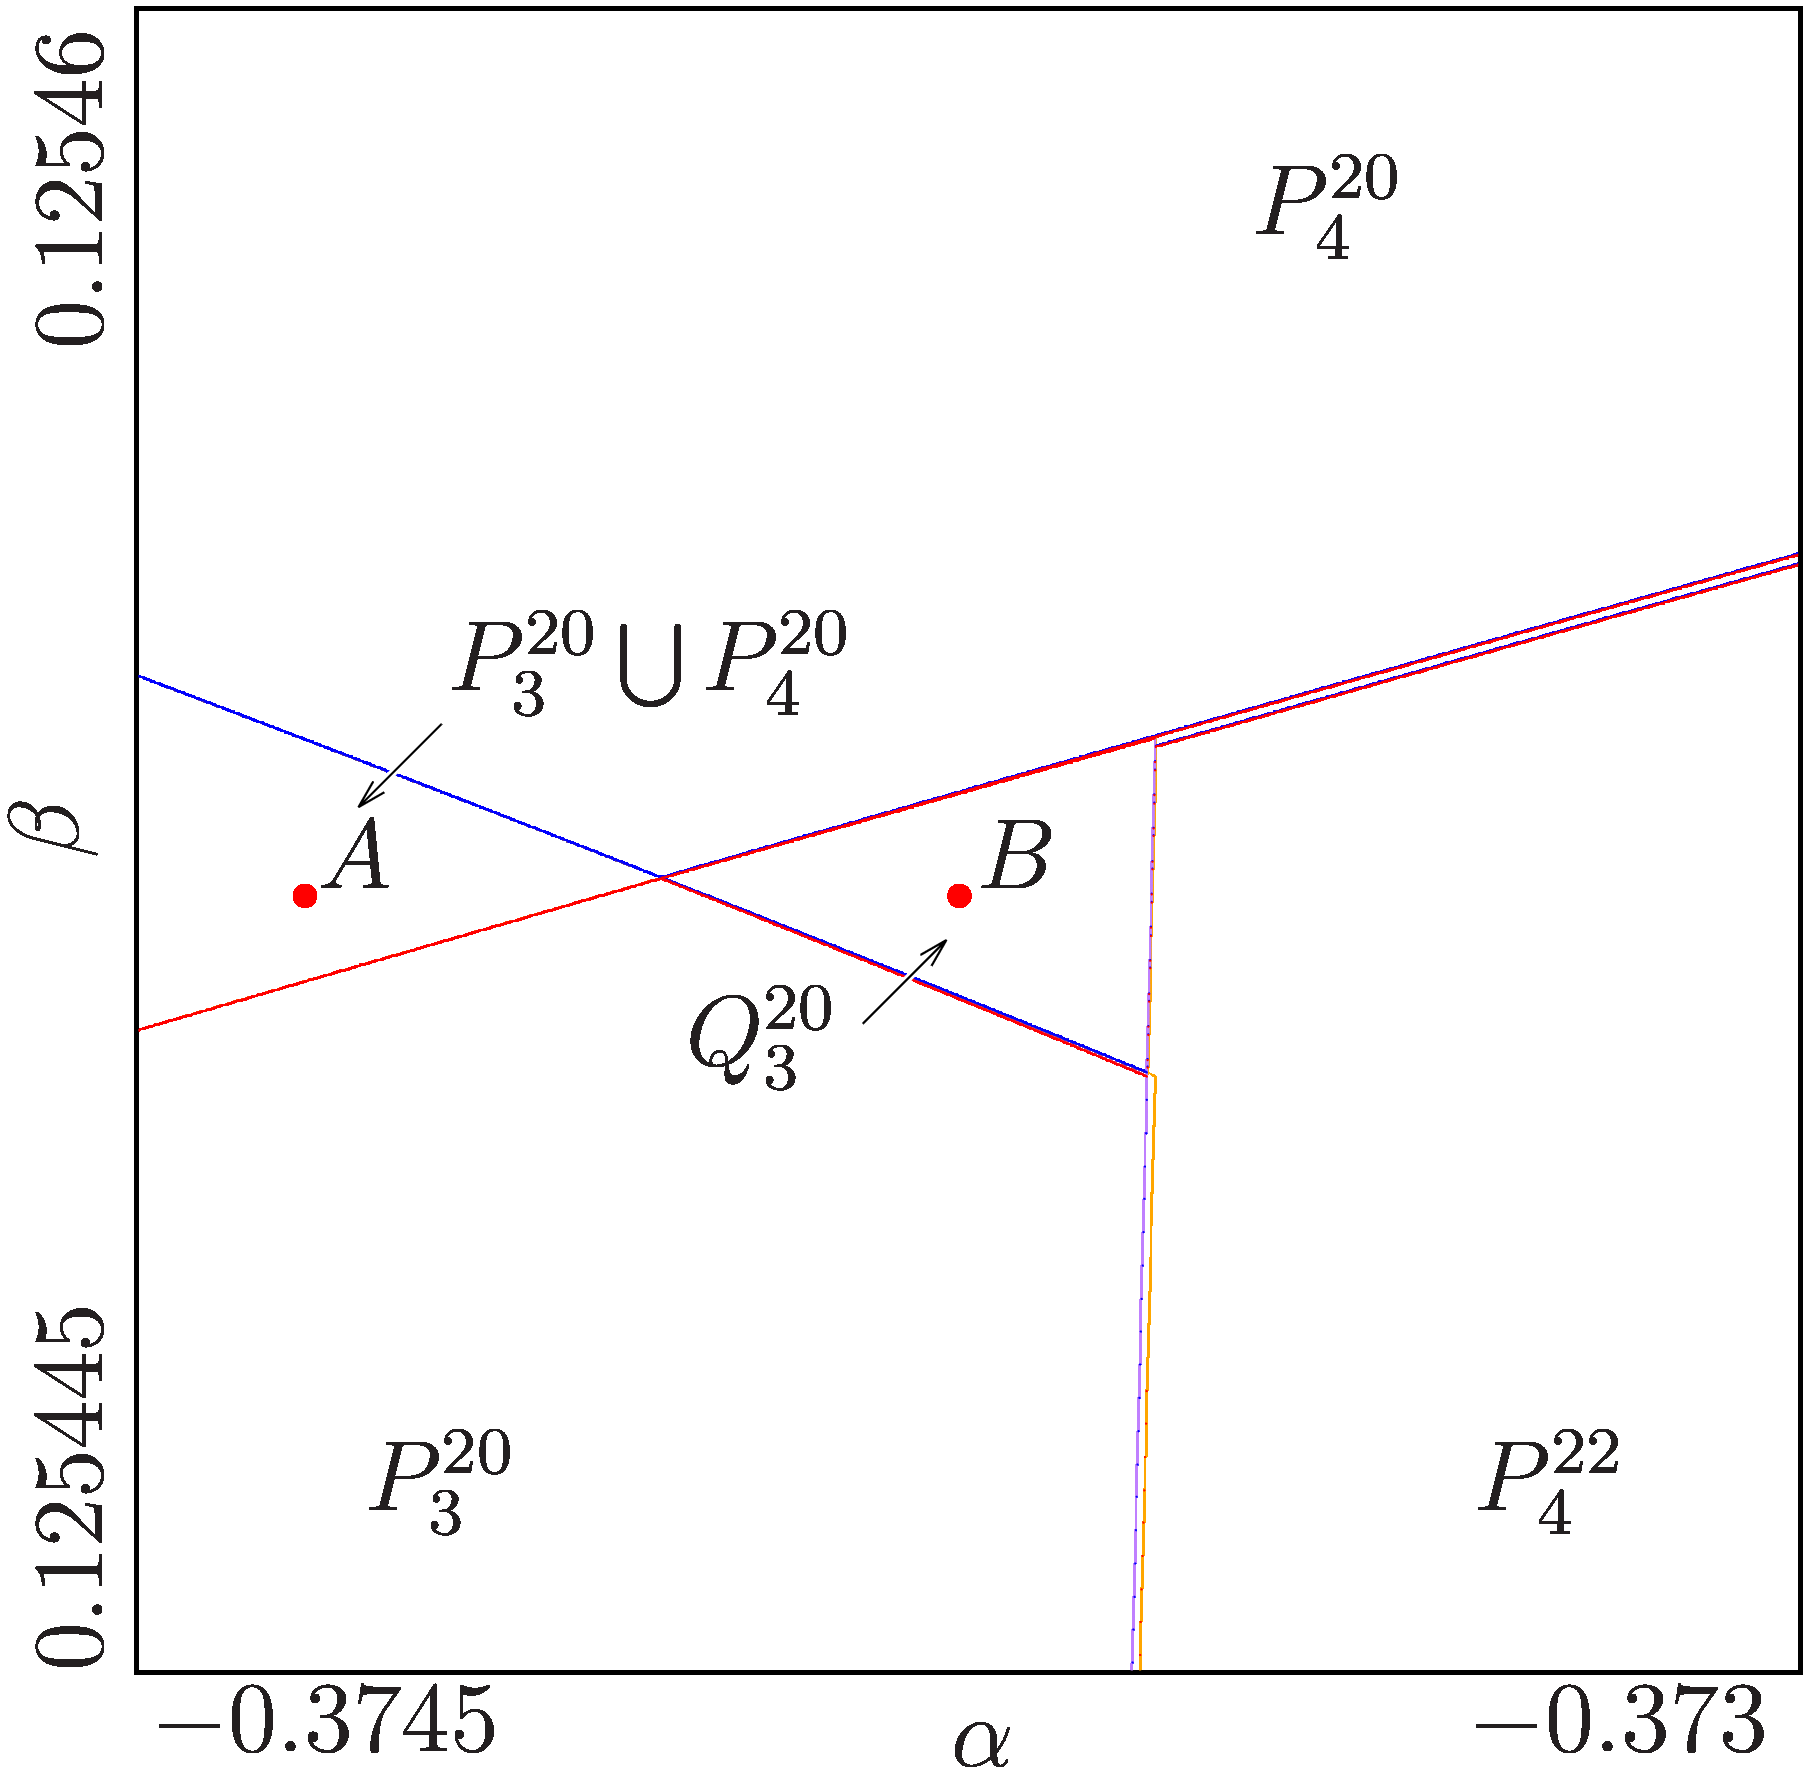
\includegraphics[width=.3 \textwidth]{../Figures/7/7.4a/result.png}
		\label{fig:add.change.disb.regions}
	}
	\subfloat[Cobweb at point $A$]{
		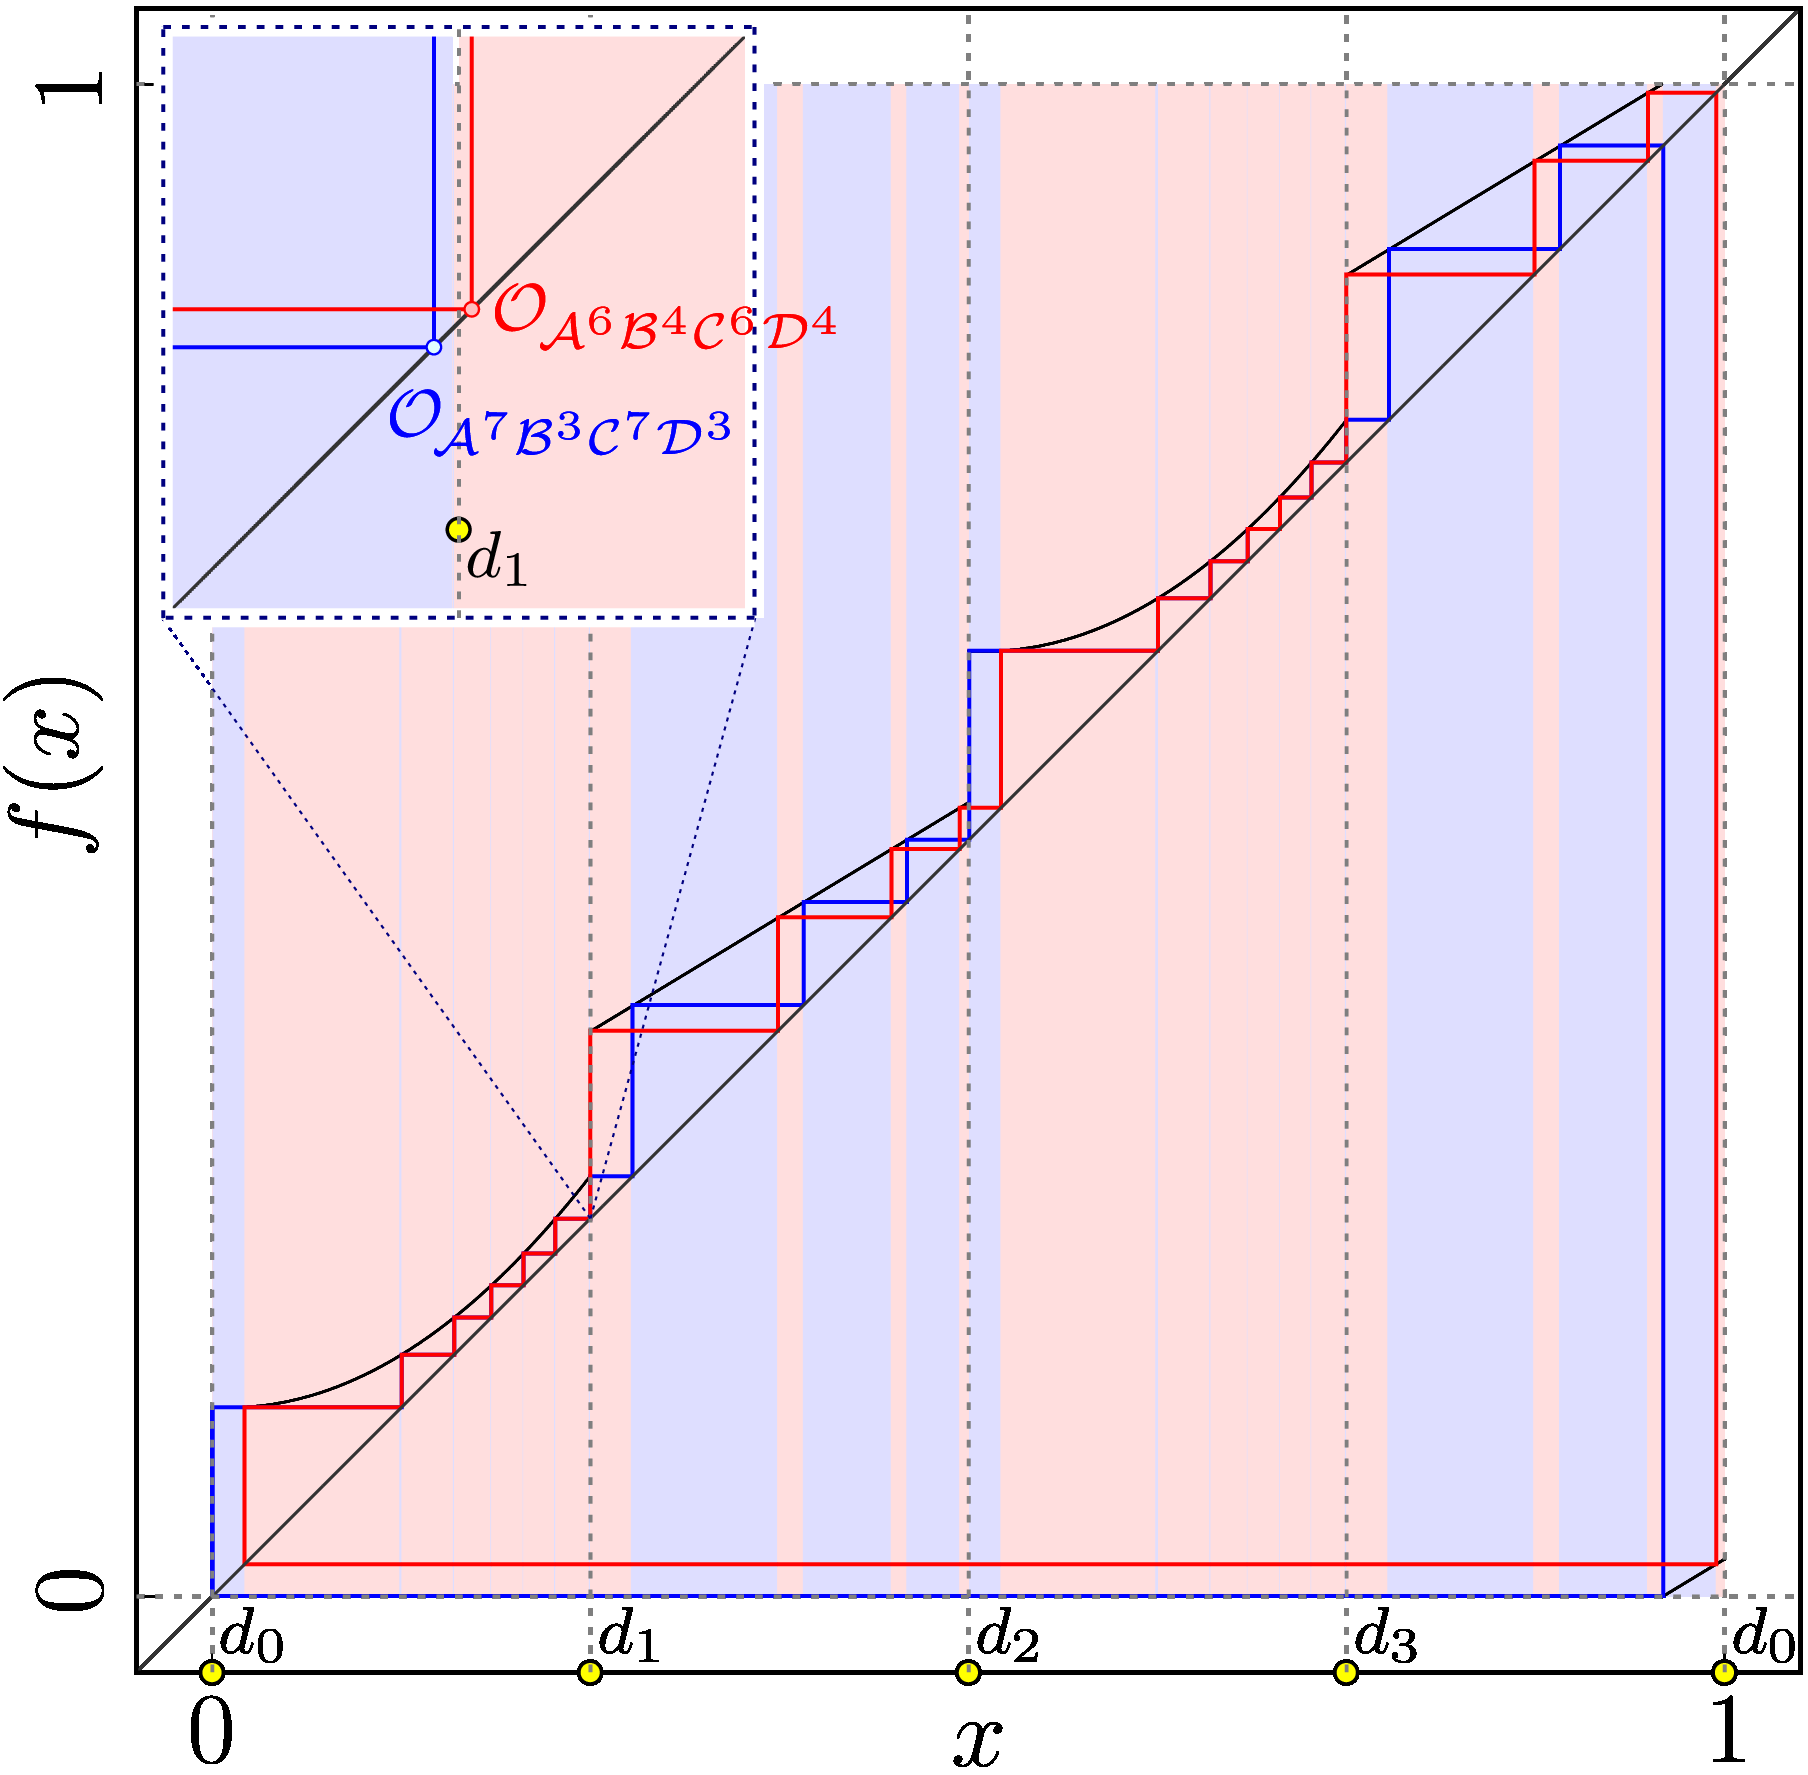
\includegraphics[width=.3 \textwidth]{../Figures/7/7.4b/result.png}
		\label{fig:add.change.disb.cob.A}
	}
	\subfloat[Cobweb at point $B$]{
		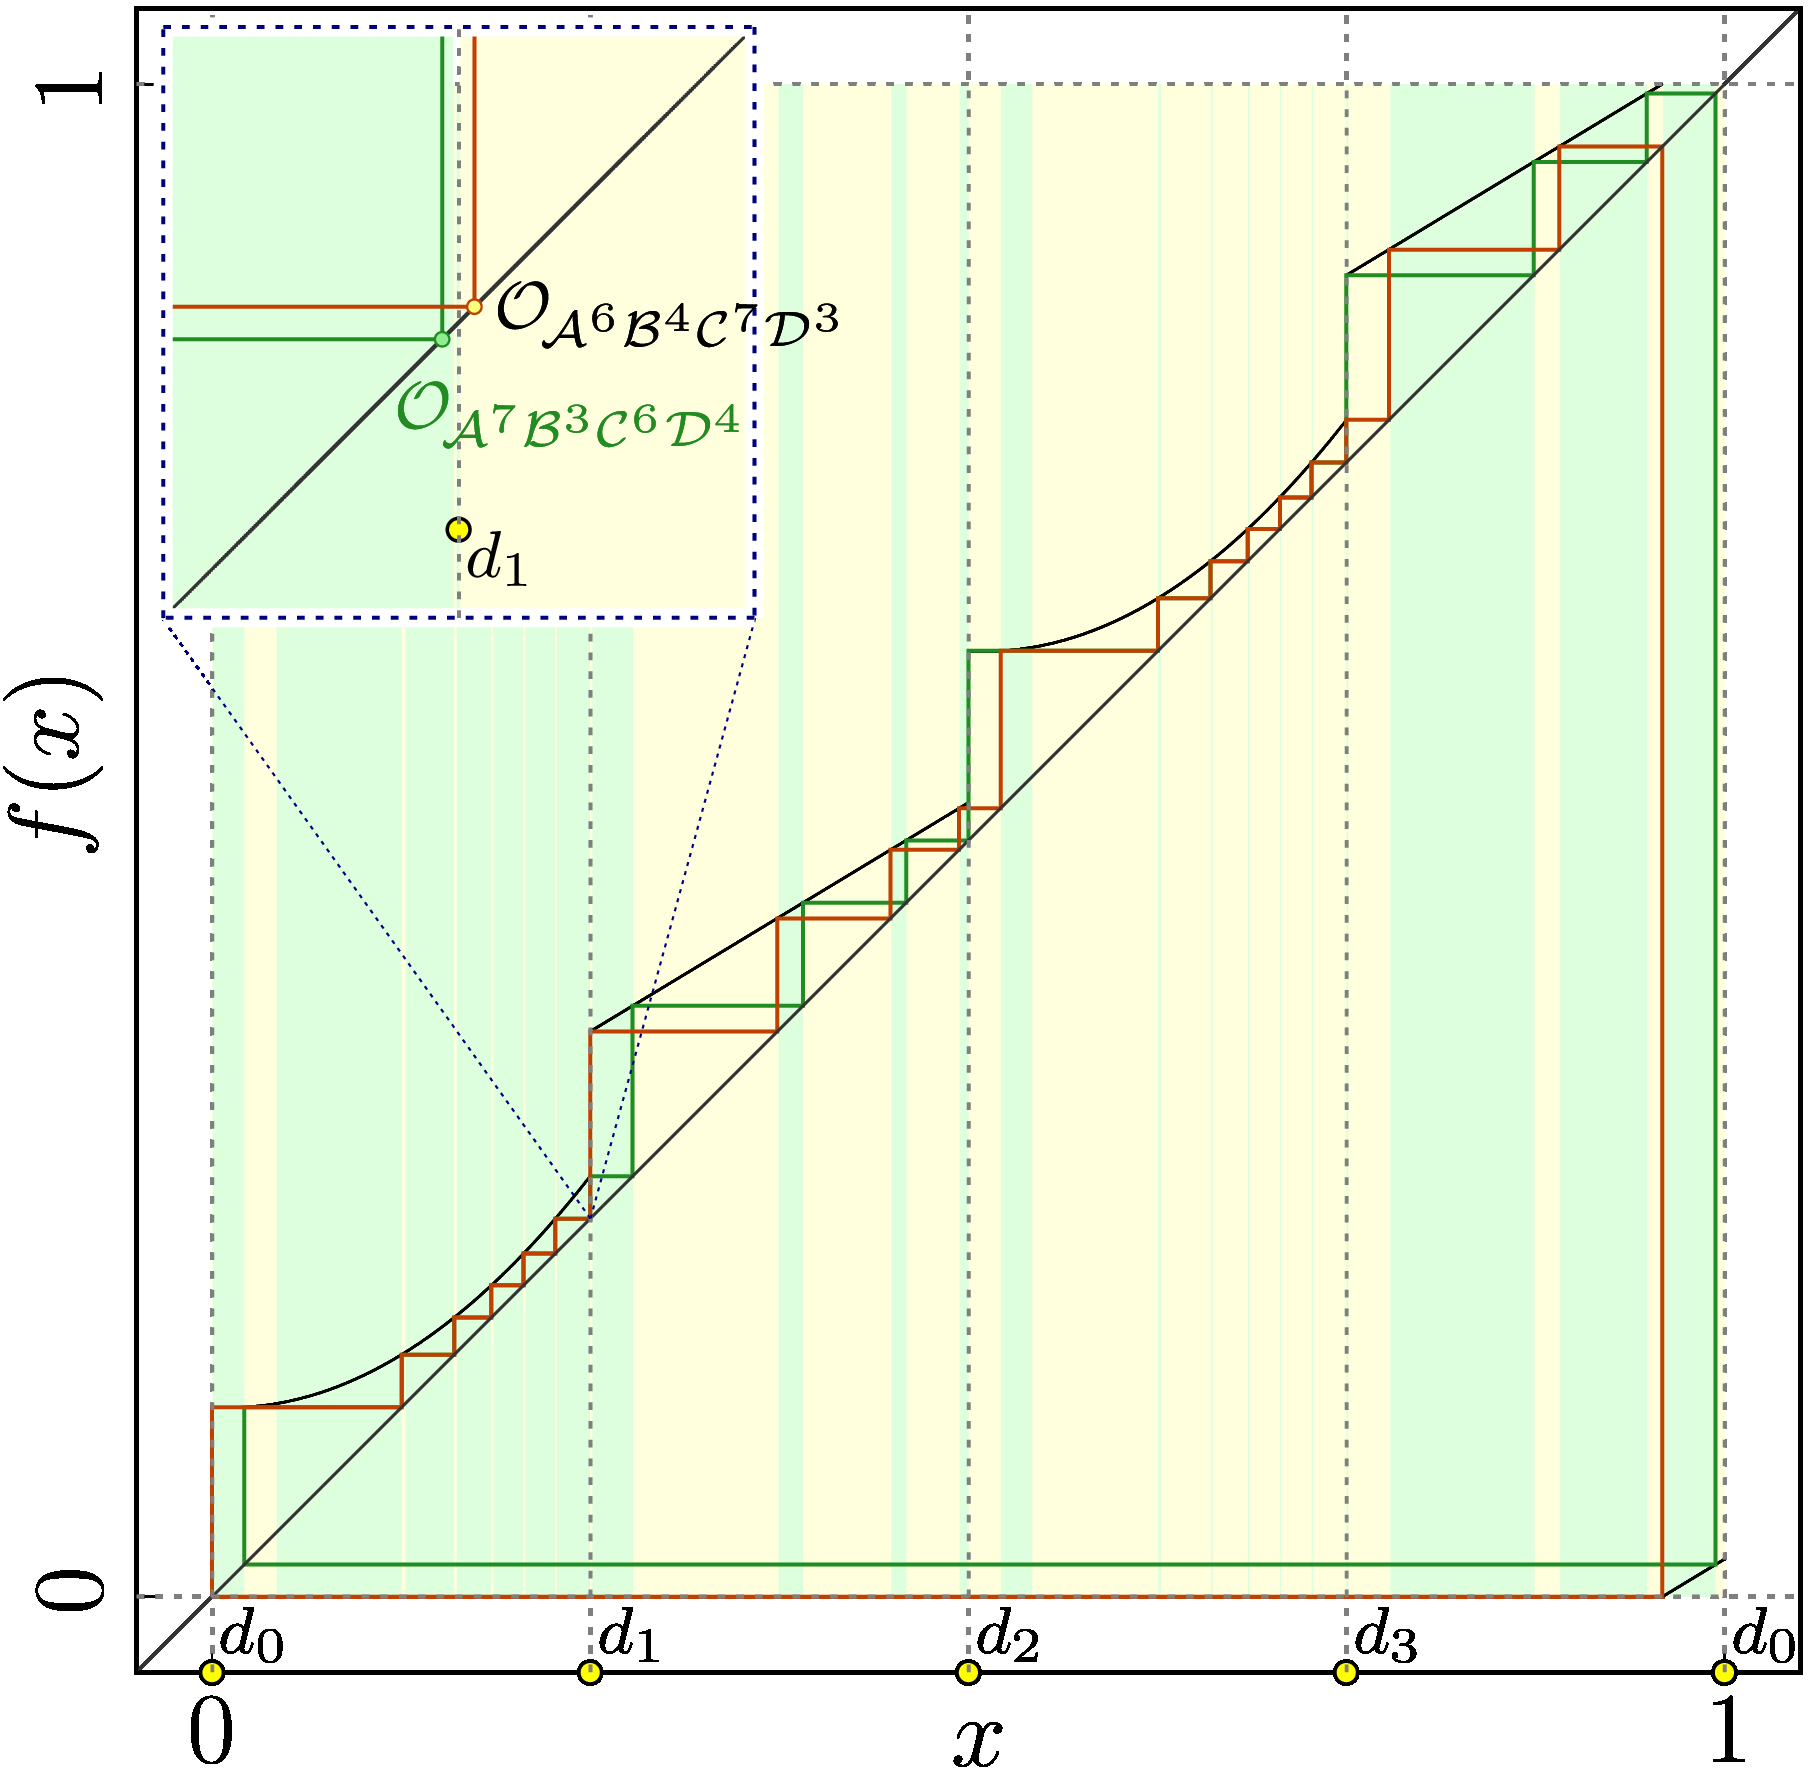
\includegraphics[width=.3 \textwidth]{../Figures/7/7.4c/result.png}
		\label{fig:add.change.disb.cob.B}
	}
	\caption{Disappearance of the ``type B'' parameter region}
\end{figure}

\Cref{fig:add.change.disb.regions} shows the same thing as \Cref{fig:add.change.regions.3} again but at parameter value closer to the diappearence of the ``type B'' parameter region.
We can see that the point where the boundaries of the ``type A'' parameter regions cross moved right and the ``type B'' parameter region got smaller.
This point is called a codimension-2 point because at this point, two bifurcations happen at the same time to the same cycle.

We know from \Cref{sec:arch.bif.sum} that the border collision bifurcation at the upper boundary of the ``type A'' parameter region $P^{20}_3$ is $\BCB_{d_1, d_3}^{\underline{\A}^7\B^3\underline{\C}^7\D^3}$.
And the border collision bifurcation at the lower boundary of the ``type A'' parameter region $P^{20}_4$ is $\BCB_{d_1, d_3}^{\A^6\underline{\B}^4\C^6\underline{\D}^4}$.
At the codimension-2 point, both these border collision bifurcations happen at the same time and both cycles vanish.
We can see in \Cref{fig:add.change.disb.cob.A} that the ``type A'' cycles are very close to the borders $d_1$ and $d_3$, respectively.

We also know that the border collision bifurcations at the upper boundary of the ``type B'' parameter region $Q^{20}_3$ are $\BCB_{d_1}^{\underline{\A}^7\B^3\C^6\D^4}$ and $\BCB_{d_3}^{\A^6\B^4\underline{\C}^7\D^3}$.
And the border collision bifurcations at the lower boundary are $\BCB_{d_3}^{\A^7\B^3\C^6\underline{\D}^4}$ and $\BCB_{d_1}^{\A^6\underline{\B}^4\C^7\D^3}$.
At the codimension-2 point, both border collision bifurcations $\BCB_{d_1}^{\underline{\A}^7\B^3\C^6\D^4}$ and $\BCB_{d_3}^{\A^7\B^3\C^6\underline{\D}^4}$ happen to the cycle $\Cycle{\A^7\B^3\C^6\D^4}$ at the same time and it vanishes.
Because of the symmetry, the border collision bifurcations $\BCB_{d_3}^{\A^6\B^4\underline{\C}^7\D^3}$ and $\BCB_{d_1}^{\A^6\underline{\B}^4\C^7\D^3}$ happen to the cycle $\Cycle{\A^6\B^4\C^7\D^3}$ at the same time and it vanishes also.

This codimension-2 point moves right with higher values for $b_L$ along the parameter line given by \Cref{equ:add.change.paramline}.
As soon as the codimension-2 point crosses the right boundary of the ``type B'' parameter region, the ``type B'' parameter region ceases to exist.
Instead, now the two ``type A'' parameter regions overlap without the codimension-2 point.
This new overlapping regions is bounded by simple ``type A'' boundary border collision bifurcations as they are discussed in \Cref{sec:arch.bif.sum}.
